\scanpage{156}
% position: top cancelled calculation
\[\deleted{-\chi(1-\delta\chi)}\]
\[\unsure{\xi|\delta}\]
% position: boxed upper formula
\[
\boxed{\begin{aligned}
&-\chi(1-\delta\chi)x_1\otimes x_2+(1-\delta\chi)[x_1\otimes\pi_2(x_2)+\pi_1(x_1)\otimes x_2)\\
&\hspace{6em}+\delta\pi_1(x_1)\otimes\pi_2(x_2)
\end{aligned}}
\]
% position: text and coefficient values below box
Si \(\chi=2\), on \unsure{peut} prendre \(\delta=1\)

donc
\[
\begin{aligned}
\alpha&=-2(1-2)=2\\
\beta&=\gamma=1-2=-1
\end{aligned}
\]
donc
\[
2x_1\otimes x_2-[(x_1\otimes\pi_2(x_2)+\pi_1(x_1)\otimes x_2)]+\pi_1(x_1)\otimes\pi_2(\unsure{x_2)}
\]
% position: middle cancelled formula
\[\deleted{\pi_i(x_i)=2x_i-T_i\psi(x_i)}\]
% position: middle bar formulas
\[
\begin{aligned}
\pi_i(x_i)&=2x_i-T_i\psi_i(x_i)=2x_i-(x_i+\bar x_i)\\
&&\hspace{9em}\unsure{x_i}-\bar x_i\\
\bar x_i&=.T_i\psi_i(x_i)-x_i\qquad\deleted{=\unsure{x}}\\[.7em]
x_i+\bar x_i&=T_i\psi_i(x_i)
\end{aligned}
\]
% position: lower tensor expansion
\[
\begin{aligned}
&2x_1\otimes x_2-[(\uline{x_1\otimes(x_2}-\bar x_2)+(x_1-\uline{\bar x_1)\otimes x_2})]
+\uline{(x_1-\bar x_1)\otimes(x_2}-\unsure{\overline{\overline{x_2}})|\bar x_2)}\\
&\qquad=x_1\otimes x_2+\bar x_1\otimes\bar x_2\qquad\text{o.K.}
\end{aligned}
\]
% position: lower left separator
\figure{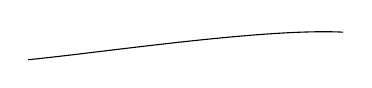
\begin{tikzpicture}\draw (0,0)..controls (1,.1) and (3,.4)..(4,.35);\end{tikzpicture}}
% position: lower unfinished bar expression
\[
\overline{\unsure{X_i|x_i}}=x_i-\pi_i(x_i)=\bigl\{
\]
% position: bottom cancelled tensor continuation
\[
x_1\otimes x_2+\deleted{(\unsure{x_1}-\unsure{\pi_1(x_1)}}
\]
% position: bottom coefficient equations
\[
\begin{gathered}
-\chi(1-\delta\chi)\overset{?}{=}\chi\\[.8em]
-1+\delta\chi=1\qquad\boxed{\delta\chi=2}\\
\unsure{:|-}
\end{gathered}
\]
% position: foot pencil
\margin{155}
